%Title 
\begin{figure}
\centering
{\Huge Model Building and Simulation (MODUS)}\\[0.5cm]
{\Huge Exercise 4}\\[0.5cm]
{\Large Alexander Rimer / Eleni Milona}\\[0.6cm]  
{\Large 1138243 / 1150221}\\[0.6cm]  
\today
\end{figure}

\section{Modeling the real-world problems}
\subsection{Simulation method}
We choose a discrete-event model, because with this kind of model:
\begin{itemize}
  	\item you can identify bottlenecks
	\item	you can vary the parameters to get forecasts of the systembehaviour
	\item	the agent behaviour is not of interest to the objectives, the process flow is
\end{itemize}

\subsection{Conceptual model}
i) 
	\textbf{Objectives:}
		\begin{itemize}	
		  \item Serve 95\% of ``normal'' customers in less than 5 minutes
		  \item Serve 99\% of ``VIP'' customers in less than 3 minutes
		\end{itemize}
ii) 	
	\textbf{Inputs:}
		\begin{itemize}	
		  \item number of customers in queue (max. 10 for ``normals'', max. 25 for VIPs)
		  \item number of employees at counter
		  \item service time (at counter)
		  \item arrival rates of customers
		\end{itemize}
		
	\textbf{Outputs:}
		\begin{itemize}	
		  %\item time: (3 and 5 minutes)
		  %\item percentage ( 99 and 95)
		  \item \% of customers queuing for less than 5 (or 3) minutes
		  \item employees utilisation
		  \item statistical outputs like histograms etc
		\end{itemize}
		
	\textbf{Content:}
		\begin{itemize}	
		  \item Employees at counter
		  \item queues of normal / VIP customers
		  \item different priorities for VIPs and ``normals''
		  \end{itemize}

iii)
\textbf{Simplification:}
	\begin{itemize}
	  \item Customers standardized (socio - economic-characteristics not of importance)
	  \item VIP - queue has  max. 10 entities
	  \item ``normals'' - queue has max. 25 entities
	  \item Customer arrival rates, time of day, different products, etc. are abstracted (not important)
	\end{itemize}
	
\textbf{Assumptions:}
	\begin{itemize}
	  \item Optimal queues: no queue-jumping, leaving etc.
	  \item Employees: attributes  (e.g. tiredness, breaks, working speed etc.) are modeled after averages or some 
	        statistical distribution
	\end{itemize}


\subsection{Conceptual model, a graphical representation}
The following shows a graphical representation of the conceptual model which is explained  in task 1.
	\begin{figure}[!htb]
  \centering   
  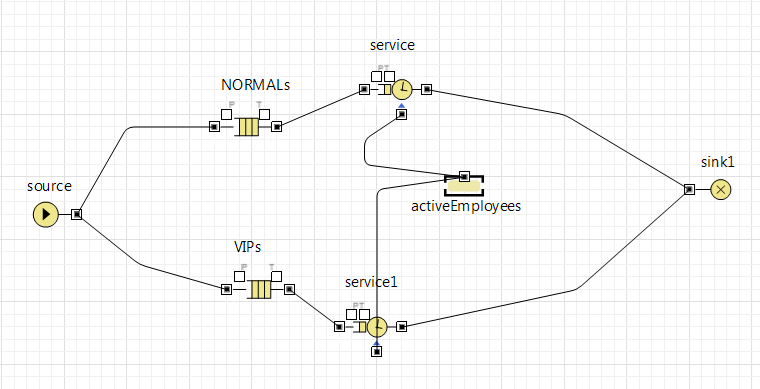
\includegraphics[width=1\textwidth]{pics/ub4/dia} 
  \caption{graphical representation of the model}
  \label{fig:dia} 
 \end{figure}

\section{Design of experiments}
How can a farmer work the best potato sort - fertilizer combination out?\\
One could use the $2^k $ expermient design where $k=2$: potato sort, fertilizer.
The farmer has to observe 4 scenarios:
\begin{itemize}
 \item potato sort 1 - fertilizer 1
\item potato sort 2 - fertilizer 1
\item potato sort 1 - fertilizer 2
\item potato sort 2 - fertilizer 2
\end{itemize}
However, the $2^k$ expermient design may be to complex; it would suffice to just compare the alternatives with
each other and choose the most succesfull combination.   